%---------------------------------------------------------------------
%
%                          Cap�tulo 6
%
%---------------------------------------------------------------------

\chapter{Testings and Results}

\begin{FraseCelebre}
\begin{Frase}
At last the long wait is over \\
The weight is off my shoulders \\
I'm taking all control, yeah
\end{Frase}
\begin{Fuente}
Thomas \& Guy-Manuel, Daft Punk
\end{Fuente}
\end{FraseCelebre}

\begin{resumen}
Some tests were applied to main platform modules for the purpose of proving their proper functionality. Main capabilities that make the valuable the platform such as power consumption or spectrum sensing features have been tested. Descriptions of the carried out tests and corresponding results are exposed in this Chapter.  
\end{resumen}

%-------------------------------------------------------------------
\section{Test Model}
%-------------------------------------------------------------------
\label{cap6:sec:testModel}
%-------------------------------------------------------------------
The purposes of testing functionalities of the platform are to prove valuable capabilities and proper functionality of modules. Characterization is not expressely required and modules must respond to operation parameters provided by manufacturers. The already described  used firmware includes several test-benches to apply. Most of the software tools employed to test the platform are extracted, at least partially, from them. For a further description on the provided tests design, cosult \ref{juanpfc}. 

Tests are simple and check bounded functions. Aspects to check are related to sleeping modes operation and current consumption, microcontroller computing capabilities, spectrum sensing features and radio interfaces, or battery charger behaviour.   

%-------------------------------------------------------------------
\section{Energy management test}
%-------------------------------------------------------------------
\label{cap6:sec:consumptionTest}
%-------------------------------------------------------------------
This test tries to bring the \ac{CNGD} under different operation modes. On the one hand, different sleeping modes and energy options for \ac{RI}s and \ac{MCU} are achieved consecutively. On the other hand, consumed current by the platform is measured at each situation. 
This test was already included at the firmware and just few changes were needed to fully carry it out. These changes suppose the functions to control the power at the \ac{RI}s and they are described at Section \ref{cap7:subsec:usbtraces}.  

8 Different situations are configured. Following description covers the initial state and sequential events happening:

\begin{itemize}
\item A situation: Initial situation. The three \ac{RI}s and the \ac{MCU} are in run mode.
\item B situation: 434 MHz \ac{RI} goes to sleep mode. 
\item C situation: Power supply at 434 MHz \ac{RI} is switch off.  
\item D situation: 868 MHz \ac{RI} goes to sleep mode.
\item E situation: Power supply at 868 MHz \ac{RI} is switch off.
\item F situation: 2.4 GHz \ac{RI} goes to sleep mode.
\item G situation: Power supply 2.4 GHz \ac{RI} is switch off.
\item H situation: \ac{MCU} goes to sleep mode.
\end{itemize} 

Consumption measures are reflected at Figure \ref{fig:cap6:energymodes}, where a graph shows how the current consumption goes down throughout the different set situations.

\figura{Bitmap/Capitulo6/consumption}{width=\textwidth}{fig:cap6:energymodes}%
{cNGD consumption at different energy modes.}

%-------------------------------------------------------------------
\section{Computing test}
%-------------------------------------------------------------------
\label{cap6:sec:computing}
%-------------------------------------------------------------------
This test intends to measure the computational cost for the management of the communication protocol stack. This could help to make a good software planification and avoid troubles interfering the application proper running. Moreover, it is important to adjust the management tasks period carefully for a good performance over communications.

For this, it will be determined how long takes the management task to be accomplished in a \ac{FFD}. Nominal clock frequency is set to 80 MHz and no network activity is considered. Management tasks are taken every 25 ms. This test is fully provided at the firmware. 

Table \ref{tab:cap6:tasktime} shows separately the measured time for \ac{RI}s and different protocol versions, Mesh and P2P. 

\begin{table}[h]
\centering
\scalebox{0.9}{
\begin{tabular}{l r r}
\hline
\hline
Management part & P2P Protocol & MiWi Protocol \\ \hline \hline
Common management &  & \\ \hline
434 MHz RI management &  & \\ \hline
868 MHz RI management &  & \\ \hline
2.4 GHz RI management &  & \\ \hline\hline
Total time & & \\ \hline \hline
\end{tabular}}

\caption{Time costs on the communication protocol management tasks.%
         \label{tab:cap6:tasktime}}
\end{table}

%-------------------------------------------------------------------
\section{Spectrum sensing test}
%-------------------------------------------------------------------
\label{cap6:sec:spectrum}
%-------------------------------------------------------------------
This test tries to show the right spectrum sensing capability of the platform since it supposes a key point for its purposes. Using two \ac{CNGD} prototypes and making use of the functions provided by the \ac{HAL}, three simple scenarios show sensing features at the three different frequency bands. All the scenarios host a device transmitting continously unicast packets at determined channels. This \ac{RF} activity is detected by the platform at different spectrum energy scans. 

First scenario is conducted over 434 MHz band. This band posses 2 available channels when using a bitrate of 119,2 kbps. Transmitting device is making use of channel 1. Figure \ref{fig:cap6:434sensing} shows the energy scan traces deployed by the firmware.
\begin{figure}[!h]
\centering
\subfloat[Before start transmitting packets.]{\label{fig:cap6:434sensingpre}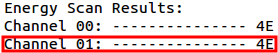
\includegraphics[height=25px]{Imagenes/Bitmap/Capitulo6/434sensingpre}}%
~
\subfloat[After start transmitting packets.]{\label{fig:cap6:434sensingpost}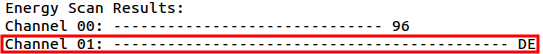
\includegraphics[height=25px]{Imagenes/Bitmap/Capitulo6/434sensingpost}}%

\caption{Spectrum sensgin at 434 MHz.}
\label{fig:cap6:434sensing}
\end{figure}


First scenario is conducted over 868 MHz band. This band posses 7 available channels when using a bitrate of 119,2 kbps. Transmitting device is making use of channel 4. Figure \ref{fig:cap6:868sensing} shows the energy scan traces deployed by the firmware.


\begin{figure}[!h]
\centering
\subfloat[Before start transmitting packets.]{\label{fig:cap6:868sensingpre}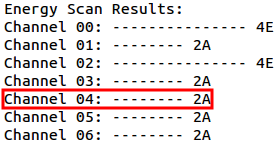
\includegraphics[height=70px]{Imagenes/Bitmap/Capitulo6/868sensingpre}}%
\qquad
\subfloat[After start transmitting packets.]{\label{fig:cap6:868sensingpost}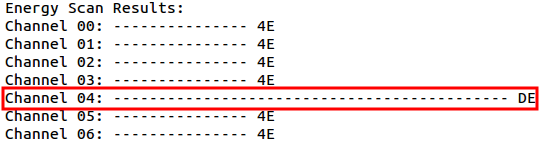
\includegraphics[height=70px]{Imagenes/Bitmap/Capitulo6/868sensingpost}}%

\caption{Spectrum sensgin at 868 MHz.}
\label{fig:cap6:868sensing}
\end{figure}

First scenario is conducted over 2.4 GHz band. This band posses 16 available channels. Transmitting device is making use of channel 4. Figure \ref{fig:cap6:2400sensing} shows the energy scan traces deployed by the firmware.

\begin{figure}[!h]
\centering
\subfloat[Before start transmitting packets.]{\label{fig:cap6:868sensingpre}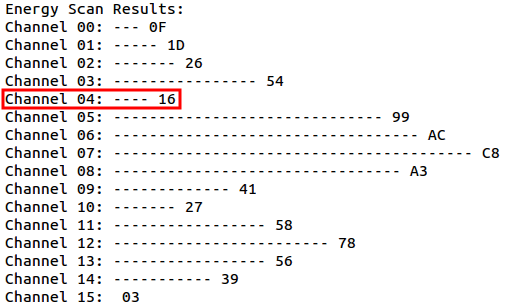
\includegraphics[height=130px]{Imagenes/Bitmap/Capitulo6/2400sensingpre}}%
~
\subfloat[After start transmitting packets.]{\label{fig:cap6:868sensingpost}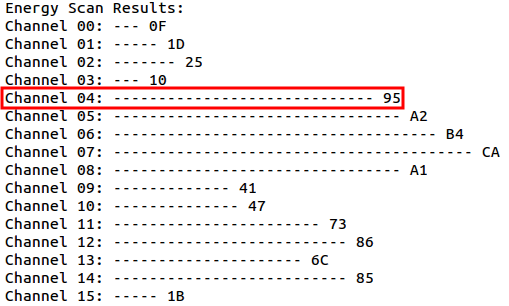
\includegraphics[height=130px]{Imagenes/Bitmap/Capitulo6/2400sensingpost}}%
\caption{Spectrum sensgin at 2.4 GHz.}
\label{fig:cap6:2400sensing}

\end{figure}

%-------------------------------------------------------------------
\section{Radio interfaces agility test}
%-------------------------------------------------------------------
\label{cap6:sec:radioagility}
%-------------------------------------------------------------------
This test evaluates how long changes over the \ac{RI}s take to be done. Parameters to change are \ac{TX} power, operation channel and energy modes. This test was fully available at the firmware. Table \ref{tab:cap6:radioagility} ilustrates the results.

\begin{table}[h]
\centering
\scalebox{0.9}{
\begin{tabular}{l r r r}
\hline
\hline
Operation & 434 MHz RI & 868 MHz RI & 2.4 GHz RI\\ \hline \hline
Switch transmission channel & 30.45 ms  &  30.4 ms & 0.151 ms \\ \hline
Change  transmission power & 55.8 $\mu$s & 55.8 $\mu$s & 70.1 $\mu$s \\ \hline
Sleep and wake up & 15.4 ms & 15.4 ms & 0.364 ms\\ \hline \hline
\end{tabular}}

\caption{Time costs on the communication protocol management tasks.%
         \label{tab:cap6:radioagility}}
\end{table}

%-------------------------------------------------------------------
\section{Effective rate test}
%-------------------------------------------------------------------
\label{cap6:sec:radiocommunication}
%-------------------------------------------------------------------
Effective rate provided by the MRF49XA and MRF24J40 transceivers driven by the firmware was already described in \cite{juanpfc}. The obtained performance must match performance achieved at the \ac{CNGD}. That is why this checking supposes a partial test compared to the full previous characterization. However, it tries new unchecked aspects of the \ac{RI}s management and proves functionality. 

Most part of this test is obtained from the firmware, so the description is covered at its literature. Employed protocol at the test-bench, for simplicity, is MiWi$^{TM}$ P2P. The three \ac{RI}s are checked and different maintenance task periods for the protocol stack are tried. In total, periods of 1 ms, 25 ms and 500 ms were tested, not obtaining performance differences among them. To avoid redundancy, shown results correspond to 25 ms period.

Two \ac{TX} modes are broadcast and unicast (long address). Main communication parameters set for the test follow:

\begin{itemize}
\item Payload size is set to 90 Bytes.
\item TX and RX buffer is configured as 10 packets for each \ac{RI}.
\item Total number of sent packets is 250.
\item VERIFY\_TRANSMIT option is enabled for MRF24J40 module.
\item \emph{ENABLE\_SECURITY} option is active.
\end{itemize}

Tables \ref{cap6:tab:effectiverate434868fast} and \ref{cap6:tab:effectiverate434868slow} ilustrate the results at two different bit-rates for $\mu$Trans module at 434 MHz and 868 MHz. Both versions, sharing the same transceiver, posses similar performance. Used protocol is P2P.  

\begin{table}[h]
\centering
\scalebox{0.9}{
\begin{tabular}{ c  c  c  c  c }
\hline
\hline
\multirow{2}{*}{TX mode} & Received  & Total & TX Time & Effective\\
  &  Packets & bits & (s) & rate (kpbs)\\ \hline \hline

Broadcast & 125 (50 \%) & 90000 & 2.88 & 31.250    \\ \hline
Unicast & 250 (100 \%) & 180000 & 7.34 & 24.511 \\ \hline \hline

\end{tabular}
}
\caption{Effective rate, received packets comparison for 434/868 RI using P2P protocol at 115200 bps .%
         \label{cap6:tab:effectiverate434868fast}}
\end{table} 


\begin{table}[h]
\centering
\scalebox{0.9}{
\begin{tabular}{ c  c  c  c  c }
\hline
\hline
\multirow{2}{*}{TX mode} & Received  & Total & TX Time & Effective\\
  &  Packets & bits & (s) & rate (kpbs)\\ \hline \hline

Broadcast & 250 (100 \%) & 180000 & 6.22 & 28.938   \\ \hline
Unicast & 250 (100 \%) & 180000 & 8.7 & 20.669 \\ \hline \hline

\end{tabular}
}
\caption{Effective rate, received packets comparison for 434/868 RI using P2P protocol at 38400 bps .%
         \label{cap6:tab:effectiverate434868slow}}
\end{table}


It is important to observe how there are not packet losses at unicast mode, and for 38400 bps there are not lost packets either when broadcasting. The reduced effective rate might be due to prototyping bad conditions, such as used corrections made with wires and raugh connections that should be better at consecutive mountings. \ac{RF} devices are very sensitive to these imperfections. On the other hand, \ac{TX} power and antenna conditions must be review, since these suposse a change with respect to previous tests.

Table \ref{cap6:tab:effectiverate2.4} ilustrates the results for MRF24J40 transceiver as 2.4 GHz \ac{RI} using a P2P protocol. 

\begin{table}[h]
\centering
\scalebox{0.9}{
\begin{tabular}{ c  c  c  c  c }
\hline
\hline
\multirow{2}{*}{TX mode} & Received  & Total & TX Time & Effective\\
  &  Packets & bits & (s) & rate (kpbs)\\ \hline \hline

Broadcast & 130 (52 \%) & 93600 & 3.25 & 28.8    \\ \hline
Unicast & 140 (56 \%) & 100800 & 3.54 & 28.474 \\ \hline \hline

\end{tabular}
}
\caption{Effective rate, received packets comparison for 2.4 GHZ RI using P2P protocol.%
         \label{cap6:tab:effectiverate2.4}}
\end{table} 

A worrying issue, already described in \cite{juanpfc}, is the packet loss even transmitting at unicast mode. The reason for this fact still remains unknown but there are some possible explanations. Most feasible option at the current moment is that \ac{ACK} packets are misinterpreted by the receiver and it considers a single \ac{ACK} response for more than one packet. This is possible due to the unsequenced character of \ac{ACK} packets at MiWi protocol. 

In order to solve this issue, Jara, G. presents in \cite{guillepfc} a flow control mechanism at MiWi \ac{MAC} layer that apparently avoid packet loss at unicast mode.

%-------------------------------------------------------------------
\section{chargerSHIELD performance test}
%-------------------------------------------------------------------
\label{cap6:sec:charger}
%-------------------------------------------------------------------
As it was mantioned, small checkings were made during the mounting process. Nevertheless, this test shows the chargerSHIELD performance test facing a battery full charge operation.

When testing the chargerSHIELD proper operation, few charging sequences were carried out. Taking measures every 2 hours of battery voltage conditions and the current flowing through it. Figure \ref{fig:cap6:chargergraph} shows the average results, battery voltages are view as blue bars referened on the left side while current flow is expressed with an orange line respect to values at the right side.

\figura{Bitmap/Capitulo6/charger}{width=\textwidth}{fig:cap6:chargergraph}%
{Batteries and parameters evolution during charging process at chargerSHIELD.}

Charging time for the defined batteries can be estimated around 12-16 hours. The ready battery led notifies the battery is ready when approximately 60\% of the total charge is available. It might be extrange to observe so high voltage values at the batteries when they are supposed to provide 3.6 V, nevertheless, it is a normal behaviour. The charger properly switchs off the charging current when voltage at the battery reveals a complete charge.


% Variable local para emacs, para  que encuentre el fichero maestro de
% compilaci�n y funcionen mejor algunas teclas r�pidas de AucTeX
%%%
%%% Local Variables:
%%% mode: latex
%%% TeX-master: "../Tesis.tex"
%%% End:
